%\documentclass[11pt,a4paper]{amsart}
\documentclass[paper=a4, fontsize=11pt]{scrartcl}
%\documentclass[12pt, final]{sreport}
\usepackage[utf8]{inputenc}
\usepackage[icelandic]{babel}
\usepackage[T1]{fontenc}
\usepackage{color}
\usepackage{amsmath, amsthm, amssymb, amsfonts}
\usepackage{enumerate}
\usepackage{url}
\usepackage{cite}
\usepackage{listings}
\usepackage{graphicx}
\usepackage{fancyhdr}
\usepackage{booktabs}
\usepackage{float}
\usepackage{hyperref}
\usepackage{caption}
\usepackage{subcaption}
\usepackage{setspace} 
\usepackage{lipsum}
\usepackage{ifthen}
\usepackage{geometry}
\usepackage{hyperref}
\usepackage{bookmark}

%\onehalfspacing
%\addtolength{\textheight}{2.4cm}
%\addtolength{\hoffset}{-1.2cm}
%\addtolength{\voffset}{-2cm}
%\addtolength{\textwidth}{2.3cm}

% Define new commands and operators
%\newcommand{\N}{\mathbb{N}}
%\newcommand{\No}{\N_0}
%\newcommand{\Z}{\mathbb{Z}}
%\newcommand{\perms}{\mathfrak{S}}

%\DeclareMathOperator{\prst}{\mathcal{P}} 
%\DeclareMathOperator{\rem}{rem}	
%\DeclareMathOperator{\id}{id}
% End of new commands definitions

% Setup theorem styles
%\theoremstyle{plain}
%\newtheorem{theorem}{Theorem}[section]
%\newtheorem{proposition}[theorem]{Proposition}
%\newtheorem{lemma}[theorem]{Lemma}
%\newtheorem{corollary}[theorem]{Corollary}
%\newtheorem{conjecture}[theorem]{Conjecture}

%\theoremstyle{definition}
%\newtheorem{definition}[theorem]{Definition}
%\newtheorem{example}[theorem]{Example}

%\theoremstyle{remark}
%\newtheorem*{remark}{Remark}
% End of theorem styles setup



\begin{document}

\newcommand{\HRule}{\rule{\linewidth}{0.5mm}}

\begin{titlepage}

\begin{center}
% Upper part of the page
%\includegraphics[width=0.55\textwidth]{rulogo.png}\\[4.0cm]    
%\includegraphics[width=4cm]{rulogo.png}

%\textsc{\LARGE Háskólinn í Reykjavík}\\[1.5cm]

\textsc{\LARGE Gagnavinnsla}\\[0.5cm]
\textsc{\Large Hópaverkefni 3}\\[0.6cm]

% Title
\HRule \\[0.4cm]
{ \Huge \bfseries Besta land í heimi}\\[0.2cm]

\HRule \\[1.5cm]


% Author and supervisor
\begin{minipage}{0.49\textwidth}
\begin{flushleft} \large
\emph{Nemandi:}\\
Arnar Ingi Halldórsson\\
Halldór Stefánsson\\
Hjörleifur G. Bergsteinsson\\
Lárus Ívar Ívarsson\\
Þór Tómasarson
\end{flushleft}
\end{minipage}
\begin{minipage}{0.49\textwidth}
\begin{flushright} \large
\emph{Kennari:} \\
Eyjólfur Ingi Ásgeirsson
\end{flushright}
\end{minipage}

\vfill

% Bottom of the page
{\large \today}



\end{center}

\end{titlepage}

\section{Aðferð/Niðurstaða}
Í þessu verkefni skoðum við gagnasöfn frá \href{http://data.worldbank.org/data-catalog/world-development-indicators}{World Bank} þar má finna WDI(CSV)-ZIP (39 MB). Eitt af markmiðum okkar var að skoða hvaða landa væri best að búa í miðað við gögn frá World Bank. Við fengum gagnasöfnin á .csv formi frá World Bank.\par Gögnin eru lesin inn í Python með 'pandas' sem við notum til að laga gögnin til þess vera viss um að þau séu á réttu formi. Gögnin vistuð í tímabundinni skrá og lesin inn í 'SQL' gagnagrunn með því að keyra 'COPY' skipunina, vegna fljótvirkni hennar, í gegnum 'psycopg2' pakka í Python sem er tengingin okkar frá Python við Postgresql gagnagrunninn. Út frá þeim gagnagrunni náum við í þau gögn sem við viljum vinna með, sjá mynd %~\ref{fig:top20}.
\par Við settum einning upp notendaviðmót þar sem notandaninn getur valið land og ákveðin gagnaflokk eins og t.d. 'Fertility rate'. Þessi gögn er hægt að rissa upp, bestu línu og tölfræði. Einnig er hægt að velja sömu gögn fyrir annað land eða önnur gögn fyrir sama land og greina hlið við hlið við fyrri gögnum. Viðmótið og viðeigandi SQL skipanir eru hannaðar með því markmiði að hægt er að uppfæra tölfuna ef nýjar tölur eru sóttar og líka er hægt að bæta við nýju stöku gagnasetti í gegnum notendaviðmótið fyrir öll löndin.


\subsection{Besta land í heimi}
Hér vildum við komast að því hvar væri best að búa miðað við þau gögn sem við höfðum í höndunum. Við völdum 10 atriði sem við notum til byggja okkar niðurstöður á:\\
\noindent

\vspace{3mm}
\noindent
%\begin{center}
-Electric power consumption (kWh per capita)\\
-Health expenditure, total (\% of GDP)\\
-Internet users (per 100 people)\\
-Life expectancy at birth, total (years)\\
-Long-term unemployment (\% of total unemployment)\\
-Mortality rate, infant (per 1,000 live births)\\
-Public spending on education, total (\% of GDP)\\
-Strength of legal rights index (0=weak to 12=strong)\\
-Tax revenue (\% of GDP)\\
-Unemployment, total (\% of total labor force)\\
\vspace{3mm}
%\end{center}
\par
Notandinn byrjar að velja ár sem hann vill skoða og ýtir á 'Best Place to Live' og þá kemur upp topplistinn fyrir það ár, sjá mynd~\ref{fig:best}
Þegar við metum einkunn landa í hverju atriði, fær efsta landið 1 í einkunn og síðan fá löndin einkunn í hlutfalli við efsta gildið. Formúlan er þá (Gildi lands/Hæsta gildi). Þar sem við erum með 10 atriði þá gefum við hverju atriði 10\%, einnig ef vil teljum að gögnin eigi að hafa neikvæð áhrif á niðurstöðuna þá margföldum við það með $ -1 $ og þar af leiðandi dregst það frá.\par
Síðan getur notandinn valið sjálfur atriði(lágmark 4), sem hann vill meta eftir til að fá sinn lista af löndum sem best er að búa í. 

\newpage

\subsection{Top tíu listi}
Þegar viðfangsefni er valið er hægt að fá top 10 lista yfir þau lönd sem eru annaðhvort verst eða best í þeim flokk. Staða landsins sem er valið kemur einnig inn á listan til samanburðar við top 10 listan. Listinn er útbúinn fyrir það ár sem er valið og einnig hvort notandinn vill fá efstu sætin eða neðstu sætin. Mynd~\ref{fig:topp}.
\\

\subsection{Uppsetning}
Forritið er keyrt með 'run.py' skipuninni. Fyrst er náð tengingu við gagnagrunninn. Næst athugar það hvort notandinn hafi nú þegar lesið gögnin inn í gagnagrunninn og flytur þau inn ef það á eftir. Þá virkjar hann 'import\_data.py' en þar finnast helstu skipanir sem við notum til að laga til gögnin í Python og koma þeim yfir í gagnagrunninn. Þar finnst skipunin 'addData' sem gerir það lítið mál að bæta við öðrum utanaðkomandi gagnasöfnum við gagnasafnið okkar.\par
Ef gagnasafnið er til nú þegar eða eftir að það hefur verið lesið inn er notandaviðmótið 'theUI.py' keyrt upp. Þar finnast helstu skipanir þar sem við náum í gögn úr gagnagrunninum. Viðmótið er hannað í Qt designer og keyrt með 'pyqt' pakkanum. Mynd~\ref{fig:gui}.

\newpage

\section{Viðauki}
\begin{figure}[H]
\begin{center}
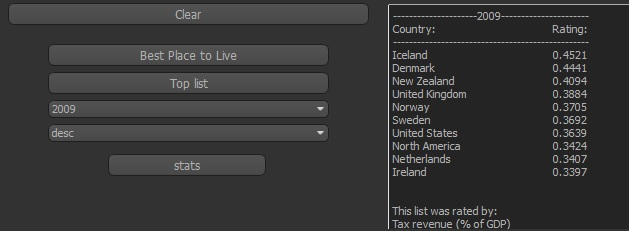
\includegraphics[height=40mm]{images/best.jpg}
\caption{$ Besti\ stadurinn\ til\ ad\ bua\ arid\ 2010 $\label{fig:best}}
\end{center}
\end{figure}

\begin{figure}[H]
\begin{center}
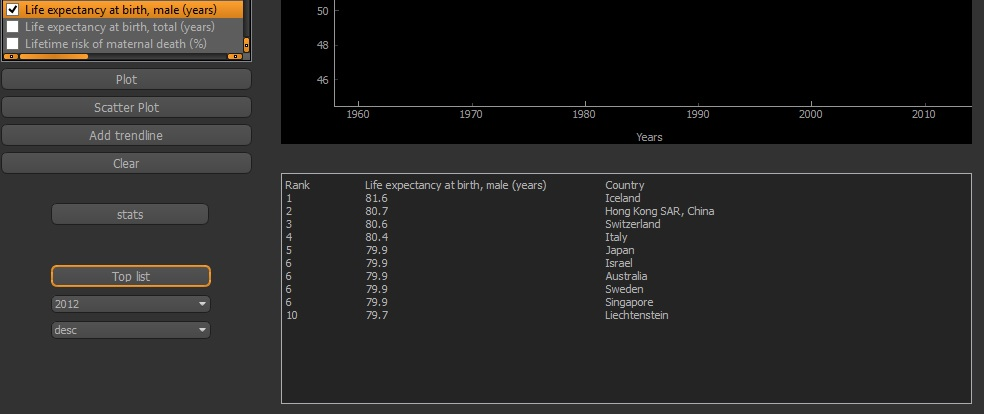
\includegraphics[height=50mm]{images/topList_life.jpg}
\caption{$ Topplisti\ fyrir\ 'Life\ Expectancy' $\label{fig:topp}}
\end{center}
\end{figure}

\begin{figure}[H]
\begin{center}
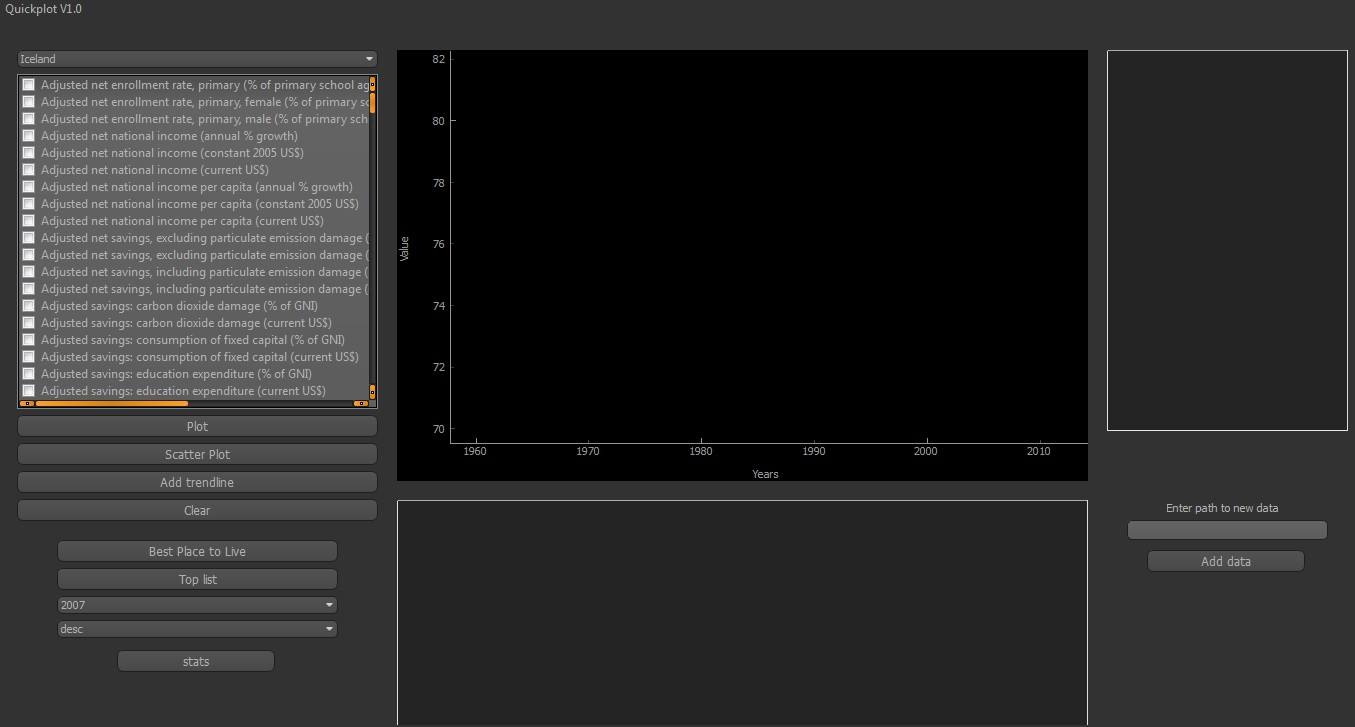
\includegraphics[height=50mm]{images/gui_front.jpg}
\caption{$ Notendavidmotid $\label{fig:gui}}
\end{center}
\end{figure}

\end{document}